\subsection{\Acl{MC}} 
The \acf{MC} method \cite{Marching2006} takes as an input a set of scalar function values on a cartesian mesh and extracts an approximate isosurface in the form of a mesh of triangles. The method starts by dividing the space into cubes with the set of points as cube vertices. On these points, the value is determined to be above or below the desired isovalue. According to which corners are set to be above or below, the corner configuration is then mapped to a polygon inside the cube, with vertices on the cube's edges. On an edge between a vertex above and a vertex below the desired isovalue, the exact location of the surface is then determined via linear interpolation and set as the polygon's vertex on that edge.

\subsubsection{The \acl{MC} cases}
Since there are 8 vertices on each cube, each above or below the isovalue (with equality falling to one of these categories), there are $2^8=256$ possible polygon configurations. However, many of these can be constructed by rotating or reflecting other polygons. There are therefore 15 base cases which represent all the surface polygons of the marching cubes. \autoref{fig:MC_basecase} shows how the polygons look like and we can notice that they are composed of \acp{tri}. 


\begin{figure}[b]
\centering
   \scalebox{0.8}{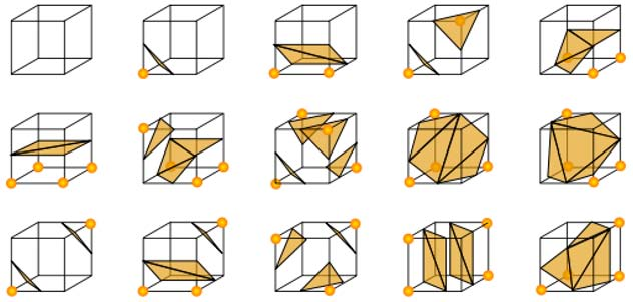
\includegraphics{Pictures/cubes.pdf}}\\
   \caption{The base cases of \ac{MC}. These are drawn with each polygon vertex intercepting its edge in the middle between the cube's corners, as in the case when the isovalue is exactly halfway between the function values at the vertices. Figure taken from \cite{Marching2006}.}
   \label{fig:MC_basecase}
\end{figure}

\subsubsection{Cracks and ambiguities}
The original algorithm presents two main problems. Firstly, it does not guarantee neither correctness nor topological consistency, which means that holes may appear on the surface due to inaccurate base case selection. Second, another problem is ambiguity, which appears when two base cases are possible and the algorithm chooses the incorrect one. There are many extended \ac{MC} algorithms that tackle the problems of the original one, getting rid of the ambiguities and providing correctness (see for example \cite{ExtendedMC}).
